\section{Environnement de Reinforcement Learning}

\subsection{Différents cas de figures}
Pour entraîner notre agent, il nous a fallu définir le contexte dans lequel nous allions l’entraîner.
Nous nous sommes placé dans deux situations :
Dans la première, le robot doit atteindre un point de l’espace avec un simple réseau de neurones : 

\begin{figure}[H]
    \centering
    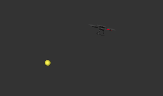
\includegraphics[width=0.5\textwidth]{./image_RL/image24.png}
    \caption{Simulation 1}
\end{figure}

Dans ce cas de figure l’agent prend pour état les distances sur XYZ pour choisir qu’elles actions réalisées. 

Dans le deuxième cas, nous avons considéré une plateforme mobile sur laquelle doit se poser le robot. Le robot dispose d’une caméra sous lui. On se sert des frames du flux vidéo pour caractériser l’état du robot.

\begin{figure}[H]
    \centering
    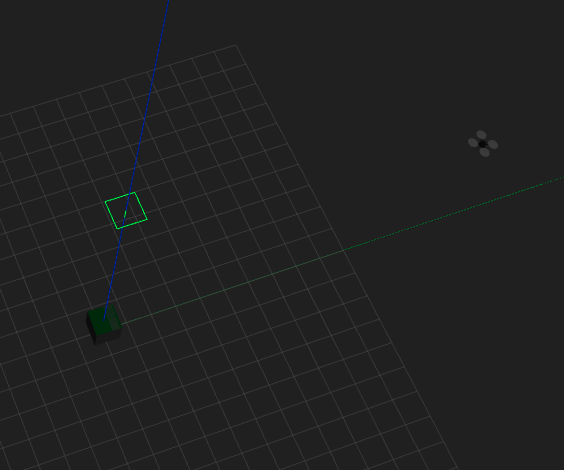
\includegraphics[width=0.5\textwidth]{./image_RL/image3.png}
    \caption{Simulation 2}
\end{figure}

\subsection{Reward function}
Dans les problèmes de reinforcement learning la fonction de reward est très importante puisqu’elle définit le MDP que l’agent doit apprendre.
Dans notre cas, la fonction de reward est assez simple.
La reward associée à une action et la différence entre les distances séparant le point du robot entre les instant t et t+1. 
Cette fonction traduit à l’agent comment il s’est déplacé par rapport à la cible en fonction de l’action qu’il a prise.

\subsection{Setup}

En reinforcement, on parle de setup pour définir les conditions d’entraînement du robot. En effet, dans un premier temps il convient de lancer l'exploration de l’agent dans un environnement où il va pouvoir apprendre réellement quelque chose.
C’est pour cela qu’il faut contraindre l’environnement d’exploration à certaines zones.
On retrouve cette problématique dans les simulations proposées par Open AI pour faire du reinforcement learning.
En effet, dans notre cas on comprend que si le robot se déplace très loin de la target il ne pourra plus apprendre beaucoup de choses. Lorsque le robot se trouve à une très grande distance, son état ne va quasiment pas évoluer quelque soit l’action qu’il réalise.
On contraint donc la zone d’exploration.
Aussi il est difficile d’entraîner l’agent en même temps que de faire la simulation, donc chaque tour de boucle nous stoppons la simulation gazebo avec les services ros de façon à attendre que l’agent ait fini son entraînement.
